\section{Predição Linear e Modelo Autorregressivo}

\begin{frame}%[allowframebreaks]
  \frametitle{Predição Linear e Modelo Autorregressivo}

  Os problemas de predição linear e modelo autorregressivo são problemas diferentes 
  que compartilham solução numérica. Em ambos os casos, deseja-se encontrar os parâmetros
  de um filtro linear. 

  No caso da predição linear (LPC), desejamos encontrar um filtro FIR
  para prever, a partir de amostras passadas, as amostras futuras de um processo autorregressivo.
  O erro encontrado é chamado erro de predição (idealmente um ruído branco).

  No caso do modelo autorregressivo, busca-se determinar o filtro IIR que,
  quando excitado por um ruído branco, produza na saída um sinal com as mesmas características
  estatísticas que o modelo que estamos buscando modelar.
\end{frame}

\subsection{Modelo Autorregressivo}
\begin{frame}%[allowframebreaks]
  \frametitle{Modelo Autorregressivo}
  Modelo Autorregressivo (AR), no contexto de processamento de sinais,
  é visto como um filtro de resposta ao impulso infinita (IIR), ou seja,
  um filtro com apenas pólos. Na física, é visto como um modelo de máxima entropia.
  Ele possui 'memória' ou realimentação, e desta forma o sistema é capaz de gerar uma
  dinâmica interna. 
\end{frame}

\begin{frame}%[allowframebreaks]
  \frametitle{Modelo Autorregressivo de Primeira Ordem}
  Modelo de primeira ordem:
  \begin{equation}
  \label{eq-1-ar}
  X_t = \varphi X_{t-1} + \mathcal{E}_t , \quad \quad \mathcal{E}_t \sim iid(0,\sigma^2)
  \end{equation}
  
  Exemplo: variação do preço do petróleo ($\Delta P_t$) em um determinado instante.
  \begin{equation}
  \Delta P_t = \frac{1}{2} \Delta P_{t-1} + \mathcal{E}_t
  \end{equation}
  onde $\mathcal{E}$ é um fator externo.
  
  Observe que o efeito de uma pertubação dura por muito tempo, diferentemente
  de um processo de média móvel em que o efeito da pertubação passa rapidamente.
\end{frame}


\begin{frame}[allowframebreaks]
  \frametitle{Modelo Autoregressivo de Primeira Ordem - Estacionário em Média}
  Dizemos que um processo é estacionário em média quando
  \begin{equation}
  E[X_t] = \textmd{const.}
  \end{equation}
  
  Para um processo de primeira ordem, dado pela Equação \ref{eq-1-ar}, teremos
  \begin{eqnarray}
  X_t &=& \varphi X_{t-1} + \mathcal{E}_t \nonumber \\
      &=& \varphi \left( \varphi X_{t-2} + \mathcal{E}_{t-1} \right) + \mathcal{E}_t \nonumber \\
      &=& \varphi^2 X_{t-2} + \varphi \mathcal{E}_{t-1} + \mathcal{E}_t \nonumber \\
      &\vdots& \\
      &=& \varphi^t X_{0} + \sum_{i=0}^{t-1} \varphi^i \mathcal{E}_{t-i} + \mathcal{E}_t
  \end{eqnarray}
  
  Qual é o valor esperado de $X_t$?
  \begin{eqnarray}
  E[X_t] &=& E\left[ \varphi^t X_{0} + \sum_{i=0}^{t-1} \varphi^i \mathcal{E}_{t-i} + \mathcal{E}_t \right] \nonumber \\
         &=& \varphi^t E\left[ X_{0} \right] + \sum_{i=0}^{t-1} \varphi^i \bcancelto{0}{E\left[ \mathcal{E}_{t-i} \right]} + \bcancelto{0}{E\left[ \mathcal{E}_{t} \right]} \nonumber \\
         &=& \varphi^t E\left[ X_{0} \right] .
  \end{eqnarray}
  Para que $E[X_t] = \varphi^t E[ X_{0}]$ seja constante devemos ter
  \begin{enumerate}
        \item $\varphi = 0$ (solução trivial), o que não desejamos; ou
        \item $E[X_{0}] = 0$, e desta forma, valor esperado de $X_t$ nulo, $\forall t$.
  \end{enumerate}
\end{frame}


\begin{frame}[allowframebreaks]
  \frametitle{Modelo Autorregressivo de Primeira Ordem - Estacionário em Variância}
  Dizemos que um processo é estacionário em variância quando
  \begin{equation}
  \textmd{var}(X_t) = \textmd{const.}
  \end{equation}
  
  Utilizando a seguinte propriedade da variância: 
  $\textmd{var}(aX) = a^2 \textmd{var}(X)$, teremos
  \begin{eqnarray}
  \textmd{var}(X_t) &=& \textmd{var}(\varphi X_{t-1} + \mathcal{E}_t) \nonumber \\
                    &=& \textmd{var}(\varphi X_{t-1}) +  \textmd{var}(\mathcal{E}_t) \nonumber \\
                    &=& \varphi^2 \textmd{var}(X_{t-1}) + \sigma^2
  \end{eqnarray}
  
  Queremos que $\textmd{var}(X_{t}) = \textmd{var}(X_{t-1}) = \textmd{var}(X_{t-2}) = \ldots$

  Teremos então
  \begin{eqnarray}
  \textmd{var}(X_t) &=& \varphi^2 \textmd{var}(X_{t-1}) + \sigma^2 \nonumber \\
                    &=& \varphi^2 \textmd{var}(X_{t}) + \sigma^2 \nonumber \\
                    &=& \frac{\sigma^2}{1 - \varphi^2}
  \end{eqnarray}
  Teremos que ter $\vert \varphi \vert < 1$ por dois motivos
  \begin{enumerate}
        \item se $\vert \varphi \vert > 1$, teríamos variância negativa, o que não
        faz sentido;
        \item se $\vert \varphi \vert = 1$ teríamos variância infinita, o que também
        não faz sentido.
\end{enumerate}
\end{frame}

\begin{frame}[allowframebreaks]
  \frametitle{Modelo Autorregressivo de Ordem $p$}
  AR(p) : modelo autorregressivo de ordem $p$
  
  \begin{equation}
  X_t = c + \sum_{i=1}^p \varphi_i X_{t-i} + \mathcal{E}_t
  \end{equation}
  
  \begin{description}
        \item[$\varphi_1, \varphi_2, \ldots, \varphi_p$] são os parâmetros do modelo
         \item[c] constante, geralmente omitida
         \item[$\mathcal{E}_t$] ruído branco
\end{description}

   Um modelo autorregressivo pode ser visto como a saída de
   um filtro de resposta ao impulso infinita (IIR) com apenas polos
   quando a entrada é um ruído branco.

  \begin{figure}[ht]
    \centering
    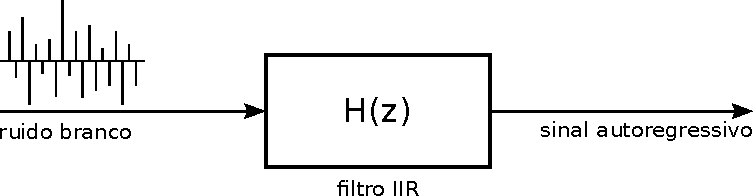
\includegraphics[width=0.5\textwidth]{images/ar-iir-filter.pdf}
    \caption{Modelo autorregressivo.}
    \label{fig:ar-iir-filter}
  \end{figure}

  \begin{eqnarray}
  H(z) &=& \frac{1}{1 - \varphi_{1} z^{-1} - \varphi_{2} z^{-2} - \ldots - \varphi_{p} z^{-p}}    \nonumber \\
       &=& \frac{1}{1 - \sum_{i=1}^{p} \varphi_{i} z^{-i}}
  \end{eqnarray}

  Para que o modelo AR(p) seja estacionário no sentido amplo 
  (ou seja, suas características estatísticas não mudam com o tempo), 
  as raízes do
  polinômio $z^p - \sum_{i=1}^{p} \varphi_{i} z^{p-i}$ devem estar dentro do
  círculo unitário, i.e. cada raiz $z_i$ deve satisfazer $\vert z_i \vert <1$.
\end{frame}


\subsection{Determinação do Modelo}
\begin{frame}[allowframebreaks]
  \frametitle{Inversão Direta}
  Vamos assumir que uma série temporal com média nula $\{x_t\}_{0}^{N-1}$
  é um processo AR e o modelo é
  \begin{equation}
        X_{t} = \varphi_1 X_{t-1} + \varphi_2 X_{t-2} + \ldots + \varphi_p X_{t-p} + \mathcal{E}_t
  \end{equation}
\end{frame}

\subsection{Inversão Direta}
\begin{frame}[allowframebreaks]
  \frametitle{Inversão Direta - $p=1$}
  No caso em que $p=1$, teremos
  \begin{equation}
        x_{t} = \varphi_1 x_{t-1} + \mathcal{E}_t
  \end{equation}

  \begin{equation}
  \begin{bmatrix} x_1 \\ x_2 \\ \vdots \\ x_{N-1}\end{bmatrix}
  = \varphi_1 \begin{bmatrix} x_0 \\ x_1 \\ \vdots \\ x_{N-2}\end{bmatrix} 
  \end{equation}
  
  \begin{eqnarray}
  \mathbf{b} &=& \varphi_1 \mathbf{A} \nonumber \\
             &=& \mathbf{A} \varphi_1
  \end{eqnarray}
 
  \framebreak 
  \begin{eqnarray}
  \mathbf{A} \hat{\varphi_1} &=& \mathbf{b} \nonumber \\
  \mathbf{A}^T \mathbf{A} \hat{\varphi_1} &=& \mathbf{A}^T \mathbf{b} \nonumber \\
  (\mathbf{A}^T \mathbf{A})^{-1} \mathbf{A}^T \mathbf{A} \hat{\varphi_1} &=& (\mathbf{A}^T \mathbf{A})^{-1} \mathbf{A}^T \mathbf{b} \nonumber \\
  \hat{\varphi_1} &=& (\mathbf{A}^T \mathbf{A})^{-1} \mathbf{A}^T \mathbf{b} 
  \end{eqnarray}
  
  \vspace{-4ex}
  \begin{eqnarray}
  \hat{\varphi_1} &=& \underbrace{(\mathbf{A}^T \mathbf{A})^{-1}}_{\left( \sum_{i=0}^{N-2} x_i^2 \right)^{-1} } \quad \underbrace{\mathbf{A}^T \mathbf{b}}_{\sum_{i=0}^{N-2}x_i x_{i+1}} \nonumber \\
  &=& \left( \sum_{i=0}^{N-2} x_i^2 \right)^{-1} \sum_{i=0}^{N-2}x_i x_{i+1} \nonumber \\
  &=& c_0^{-1} c_1 = r_1
  \end{eqnarray}
  onde $c_i$ é o $i$-ésimo coeficiente de auto covariância e $r_i$ o $i$-ésimo
  coeficiente de autocorrelação.
\end{frame}

\begin{frame}[allowframebreaks]
  \frametitle{Inversão Direta - $p=2$}
  No caso em que $p=2$, teremos
  \begin{equation}
        x_{t} = \varphi_1 x_{t-1} + \varphi_2 x_{t-2} + \mathcal{E}_t
  \end{equation}
  
  \begin{equation}
  \begin{bmatrix} x_2 \\ x_3 \\ \vdots \\ x_{N-1}\end{bmatrix}
  = \begin{bmatrix} x_1 & x_0 \\ x_2 & x_1 \\ \vdots & \vdots \\ x_{N-2} & x_{N-3}\end{bmatrix} \begin{bmatrix}\varphi_1 \\ \varphi_2\end{bmatrix} 
  \end{equation}
  
  \begin{equation}
  \mathbf{b} = \mathbf{A} \mathbf{\varphi}
  \end{equation}
  
  \begin{eqnarray}
  \mathbf{A} \hat{\mathbf{\varphi}} &=& \mathbf{b} \nonumber \\
  \mathbf{A}^T \mathbf{A} \hat{\mathbf{\varphi}} &=& \mathbf{A}^T \mathbf{b} \nonumber \\
  (\mathbf{A}^T \mathbf{A})^{-1} \mathbf{A}^T \mathbf{A} \hat{\mathbf{\varphi}} &=& (\mathbf{A}^T \mathbf{A})^{-1} \mathbf{A}^T \mathbf{b} \nonumber \\
  \hat{\mathbf{\varphi}} &=& (\mathbf{A}^T \mathbf{A})^{-1} \mathbf{A}^T \mathbf{b} 
  \end{eqnarray}
  
  \newpage
  \begin{equation}
  \hat{\mathbf{\varphi}} = (\mathbf{A}^T \mathbf{A})^{-1} \mathbf{A}^T \mathbf{b} ,
  \end{equation}
  onde
  \begin{eqnarray}
  (\mathbf{A}^T \mathbf{A})^{-1} &=& \begin{bmatrix} \begin{bmatrix} x_1 & x_2 & \ldots & x_{N-2} \\ x_0 & x_1 & \ldots & x_{N-3} \end{bmatrix} \begin{bmatrix}x_1 & x_0 \\ x_2 & x_1 \\ \vdots & \vdots \\ x_{N-2} & x_{N-3}\end{bmatrix} \end{bmatrix}^{-1}_{2\times 2} \nonumber \\
  &=& \begin{bmatrix} \sum_{i=1}^{N-2}x_i^2  & \sum_{i=1}^{N-2}x_i x_{i-1} \\ \sum_{i=1}^{N-2} x_i x_{i-1} & \sum_{i=0}^{N-3}x_i^2 \end{bmatrix}^{-1}_{2\times 2}
  \end{eqnarray}

  Se $\det(\mathbf{A}) \neq 0$, então podemos obter $\mathbf{A}^{-1}$ da seguinte forma:
  \begin{equation}
        \mathbf{A}^{-1} = \frac{1}{\det(\mathbf{A})} \text{adj}(\mathbf{A})
  \end{equation}
  onde a matriz adjunta ($\text{adj}(\mathbf{A})$) é a transposta da
  matriz de cofator $\mathbf{C}$ de $\mathbf{A}$.
  
  \begin{equation}
        C_{ij} = (-1)^{i+j} M_{ij}
  \end{equation}
  sendo $M_{ij}$ o menor $ij$ da matriz $\mathbf{A}$, ou seja, 
  o determinante da submatriz quadrada, obtida a partir de $\mathbf{A}$ 
  pela remoção da sua $i$-ésima linha e $j$-éssima coluna. 
  
  Teremos assim
  \begin{eqnarray}
  (\mathbf{A}^T \mathbf{A})^{-1} &=& \frac{1}{\det(\mathbf{A}^T \mathbf{A})} \text{adj}(\mathbf{A}^T \mathbf{A}) \nonumber \\
  &=& \frac{1}{\sum_{i=1}^{N-2}x_i^2 \sum_{i=0}^{N-3}x_i^2 - \sum_{i=1}^{N-2}x_i x_{i-1} \sum_{i=1}^{N-2} x_i x_{i-1}} \nonumber \\
  & & \begin{bmatrix} \sum_{i=0}^{N-3} x_i^2 & -\sum_{i=1}^{N-2} x_i x_{i-1} \\ -\sum_{i=1}^{N-2}x_i x_{i-1} & \sum_{i=1}^{N-2} x_i^2 \end{bmatrix}
  \end{eqnarray}
  
  Utilizando o fato de que temos uma série temporal estacionária,
  os elementos de auto-covariância são função apenas do atraso, e
  não dos limites temporais exatos. Poderemos então escrever
  \begin{eqnarray}
  (\mathbf{A}^T \mathbf{A})^{-1} &=& \frac{1}{c_0^2 - c_1^2} \begin{bmatrix} c_0 & -c_1 \\ -c_1 & c_0 \end{bmatrix} \nonumber \\
  &=& \frac{1}{c_0^2 ( 1 - r_1^2)} \begin{bmatrix} c_0 & -c_1 \\ -c_1 & c_0 \end{bmatrix} \nonumber \\
  &=& \frac{1}{c_0 ( 1 - r_1^2)} \begin{bmatrix} r_0 & -r_1 \\ -r_1 & r_0 \end{bmatrix} \nonumber
  \end{eqnarray}
  onde utilizamos que $r_i = \frac{c_i}{\sigma}$ e $\sigma = c_0$ 
  (variância é o caso especial da covariância quando as duas variáveis
  são idênticas).
  
  Analisando agora $\mathbf{A}^T\mathbf{b}$.
  \begin{eqnarray}
  \mathbf{A}^T\mathbf{b} &=& \begin{bmatrix} x_1 & x_2 & \ldots & x_{N-2} \\ x_0 & x_1 & \ldots & x_{N-3} \end{bmatrix} \begin{bmatrix}x_2 \\ x_3 \\ \vdots \\ x_{N-1}\end{bmatrix} \nonumber \\
  &=& \begin{bmatrix} \sum_{i=2}^{N-1} x_i x_{i-1} \\ \sum_{i=2}^{N-1} x_i x_{i-2}\end{bmatrix} \nonumber \\
  &=& \begin{bmatrix} c_1 \\ c_2 \end{bmatrix}
  \end{eqnarray}
  onde utilizamos mais uma vez a estacionariedade da série temporal 
  em questão.
   
  Teremos então
  \begin{eqnarray}
  (\mathbf{A}^T \mathbf{A})^{-1} \mathbf{A}^T\mathbf{b} &=& \frac{1}{c_0 ( 1 - r_1^2)} \begin{bmatrix} r_0 & -r_1 \\ -r_1 & r_0 \end{bmatrix} \begin{bmatrix} c_1 \\ c_2 \end{bmatrix} \nonumber \\
  &=& \frac{1}{ 1 - r_1^2 } \begin{bmatrix} r_0 & -r_1 \\ -r_1 & r_0 \end{bmatrix} \begin{bmatrix} r_1 \\ r_2 \end{bmatrix} \nonumber \\
  &=& \frac{1}{ 1 - r_1^2 } \begin{bmatrix} 1 & -r_1 \\ -r_1 & 1 \end{bmatrix} \begin{bmatrix} r_1 \\ r_2 \end{bmatrix} \nonumber \\
  &=& \begin{bmatrix} \frac{r_1(1-r_2)}{1-r_1^2} \\ \frac{r_2 - r_1^2}{1 - r_1^2} \end{bmatrix} = \begin{bmatrix} \varphi_1 \\ \varphi_2 \end{bmatrix} = \hat{\mathbf{\varphi}}
  \end{eqnarray}
\end{frame}



\begin{frame}
  \frametitle{Inversão Direta - $p$ qualquer}
  O mesmo procedimento pode ser feito para $p$ qualquer, 
  mas ficará cada vez mais complicado.
  
  \vspace{1cm}
  Uma maneira mais simples é utilizar as Equações de Yule-Walker.
\end{frame}
  
\subsection{Equações de Yule-Walker}
\begin{frame}[allowframebreaks]
  \frametitle{Equações de Yule-Walker}
  Utilizaremos as equações de Yule-Walker para estimar os parâmetros AR
  a partir dos dados.
  \begin{itemize}
        \item Dada uma série temporal $x[n]$, podemos estimar a sequência de
        covariância $r_{xx}[k]$ para a série temporal $x[n]$ dada.
        \item Existe uma relação entre o modelo auto-regressivo e a sequência
        de covariância. Poderemos então estimar os $p$ parâmetros do modelo
        AR de ordem $p$.
        \item Para tanto, iremos resolver as equações de Yule-Walker e 
        encontrar estes parâmetros a partir de $r_{xx}[k]$.
  \end{itemize}

  \framebreak
  O método de Yule-Walker não lida com a questão da escolha da ordem do
  modelo. Isto é usualmente feito através de um balanceamento do erro
  contra o número de parâmetros no modelo. Os seguintes métodos
  são usuais:
  \begin{enumerate}
        \item Critério de informação de Akaike (\emph{Akaike information criterion}, AIC)
        \item Critério de informação Bayesiano (\emph{Bayesian information criterion}, BIC)
        \item validação cruzada (\emph{cross validation}, CV) - utiliza
        um subconjunto dos dados para estimar o modelo, outro subconjunto
        para testar os resultados e um terceiro para validar.
        \item balancear o erro quadrático (do ajuste do modelo
  aos dados) e a ordem do modelo
  \end{enumerate}
  Ao aumentar a ordem do modelos, podemos diminuir continuamente o erro,
  obtendo um modelo cada vez mais complexo, mas isto pode não agregar,
  pois o modelo obtido pode não representar bem os dados.
  
  %%%%%%%%%%%%%%%%%%%%%%%%%
  \framebreak
  
  Considere o modelo AR(p)
  \begin{equation}
  X_t = \sum_{i=1}^p \varphi_i X_{t-i} + \mathcal{E}_t
  \end{equation}
  \underline{atraso 1}:
  multiplicando ambos os lados por $X_{t-1}$ teremos
  \begin{equation}
  X_t X_{t-1} = \sum_{i=1}^p \varphi_i X_{t-i} X_{t-1} + \mathcal{E}_t X_{t-1}
  \end{equation}
  tomando o valor esperado teremos
  \begin{eqnarray}
  E\left[ X_t X_{t-1} \right] &=& E\left[ \sum_{i=1}^p \varphi_i X_{t-i} X_{t-1} + \mathcal{E}_t X_{t-1} \right] \nonumber \\
  &=& \sum_{i=1}^p \varphi_i E\left[ X_{t-i} X_{t-1} \right] + \bcancelto{0}{E\left[ \mathcal{E}_t X_{t-1} \right]} 
  \end{eqnarray} 
  Vamos utilizar $c_l = E\left[ X_{t} X_{t-l} \right]$ e $c_l = c_{-l}$. Poderemos reescrever a equação acima como
  \begin{equation}
        c_1 = \sum_{i=1}^p \varphi_i c_{i-1}
  \end{equation}
  dividindo por $c_0 = \sigma$ teremos
  \begin{equation}
        r_1 = \sum_{i=1}^p \varphi_i r_{i-1}
  \end{equation}
  
  
  %%%%%%%%%%%%%%%%%%%%%%%%%%%%%%%%%%%%%%%%%%%%%%%%%%%
  \framebreak
  modelo AR(p)
  \begin{equation}
  X_t = \sum_{i=1}^p \varphi_i X_{t-i} + \mathcal{E}_t
  \end{equation}
  \underline{atraso 2}:
  multiplicando ambos os lados por $X_{t-2}$ teremos
  \begin{equation}
  X_t X_{t-2} = \sum_{i=1}^p \varphi_i X_{t-i} X_{t-2} + \mathcal{E}_t X_{t-2}
  \end{equation}
  tomando o valor esperado teremos
  \begin{eqnarray}
  E\left[ X_t X_{t-2} \right] &=& E\left[ \sum_{i=1}^p \varphi_i X_{t-i} X_{t-2} + \mathcal{E}_t X_{t-2} \right] \nonumber \\
  &=& \sum_{i=1}^p \varphi_i E\left[ X_{t-i} X_{t-2} \right] + \bcancelto{0}{E\left[ \mathcal{E}_t X_{t-2} \right]} 
  \end{eqnarray} 
  Vamos utilizar $c_l = E\left[ X_{t} X_{t-l} \right]$ e $c_l = c_{-l}$. Poderemos reescrever a equação acima como
  \begin{equation}
        c_2 = \sum_{i=1}^p \varphi_i c_{i-2}
  \end{equation}
  dividindo por $c_0 = \sigma$ teremos
  \begin{equation}
        r_2 = \sum_{i=1}^p \varphi_i r_{i-2}
  \end{equation}
  
  

  %%%%%%%%%%%%%%%%%%%%%%%%%%%%%%%%%%%%%%%%%%%%%%%%%%%
  \framebreak
  modelo AR(p)
  \begin{equation}
  X_t = \sum_{i=1}^p \varphi_i X_{t-i} + \mathcal{E}_t
  \end{equation}
  \underline{atraso k}:
  multiplicando ambos os lados por $X_{t-k}$ teremos
  \begin{equation}
  X_t X_{t-k} = \sum_{i=1}^p \varphi_i X_{t-i} X_{t-k} + \mathcal{E}_t X_{t-k}
  \end{equation}
  tomando o valor esperado teremos
  \begin{eqnarray}
  E\left[ X_t X_{t-k} \right] &=& E\left[ \sum_{i=1}^p \varphi_i X_{t-i} X_{t-k} + \mathcal{E}_t X_{t-k} \right] \nonumber \\
  &=& \sum_{i=1}^p \varphi_i E\left[ X_{t-i} X_{t-k} \right] + \bcancelto{0}{E\left[ \mathcal{E}_t X_{t-k} \right]} 
  \end{eqnarray} 
  Vamos utilizar $c_l = E\left[ X_{t} X_{t-l} \right]$ e $c_l = c_{-l}$. Poderemos reescrever a equação acima como
  \begin{equation}
        c_k = \sum_{i=1}^p \varphi_i c_{i-k}
  \end{equation}
  dividindo por $c_0 = \sigma$ teremos
  \begin{equation}
        r_k = \sum_{i=1}^p \varphi_i r_{i-k}
  \end{equation}
  
  %%%%%%%%%%%%%%%%%%%%%%%%%%%%%%%%%%%%%%%%%%%%%%%%%%%
  \framebreak
  $\vdots$

  \vspace{3ex}
  O mesmo ponde continuar sendo feito até $k=p$.
  
  Desta forma, poderemos montar um sistema com $p$ equações e $p$ incógnitas.

  %%%%%%%%%%%%%%%%%%%%%%%%%%%%%%%%%%%%%%%%%%%%%%%%%%%
  \framebreak
  \begin{equation}
        \begin{cases} 
        r_1 = \varphi_1 r_0 + \varphi_2 r_1 + \varphi_3 r_2 + \ldots + \varphi_{p-1} r_{p-2} + \varphi_{p} r_{p-1} \\ 
        r_2 = \varphi_1 r_1 + \varphi_2 r_0 + \varphi_3 r_1 + \ldots + \varphi_{p-1} r_{p-3} + \varphi_{p} r_{p-2} \\
        \vdots \\
        r_{p-1} = \varphi_1 r_{p-2} + \varphi_2 r_{p-3} + \varphi_3 r_{p-4} + \ldots + \varphi_{p-1} r_{0} + \varphi_{p} r_{1} \\
        r_p = \varphi_1 r_{p-1} + \varphi_2 r_{p-2} + \varphi_3 r_{p-3} + \ldots + \varphi_{p-1} r_{1} + \varphi_{p} r_{0} 
         \end{cases}
  \end{equation}
  
  \framebreak
  Este sistema de equações pode ser escrito na forma matricial.
  \begin{equation}
  \begin{bmatrix}r_1 \\ r_2 \\ \vdots \\ r_{p-1} \\ r_p \end{bmatrix} = 
  \begin{bmatrix} 
  r_0 & r_1 & r_2 & \ldots & r_{p-2} & r_{p-1} \\  
  r_1 & r_0 & r_1 & \ldots & r_{p-3} & r_{p-2} \\ 
  \vdots & \vdots & \vdots & \ddots & \vdots & \vdots  \\ 
  r_{p-2} & r_{p-3} & r_{p-4} & \ldots & r_0 & r_1 \\ 
  r_{p-1} & r_{p-2} & r_{p-3} & \ldots & r_1 & r_0 
  \end{bmatrix}
  \begin{bmatrix}\varphi_1 \\ \varphi_2 \\ \vdots \\ \varphi_{p-1} \\ \varphi_p \end{bmatrix}
  \end{equation}
  
  \begin{equation}
        \mathbf{r} = \mathbf{R} \mathbf{\varphi} 
  \end{equation}
  
  Temos um problema bem posto, com uma matriz de coeficientes quadrada
  $\mathbf{R}$, i.e., o mesmo número de equações e variáveis.
  $\mathbf{R}$ é de posto cheio e simétrica. Desta forma, a existência
  de sua inversa é garantida. Assim
  \begin{equation}
        \mathbf{\varphi} = \mathbf{R}^{-1}\mathbf{r} .
  \end{equation}
  Este sistema pode ser resolvido de forma eficiente pelo algoritmo
  de Levinson-Durbin (algoritmo utilizado para resolver sistema de equações
  com matriz de Toeplitz).
  
\end{frame}


\subsection{Estabilidade}
\begin{frame}[allowframebreaks]
  \frametitle{Estabilidade e Localização dos pólos no modelo AR}
  Um modelo autorregressivo pode ser expresso em termos de uma
  sequência de inovações $\mathcal{E}_t$
  \begin{equation}
        X (z) = z^p \left( \sum_{i=0}^{p} \varphi_i z^{p-i} \right)^{-1} \mathcal{E}(z)
  \end{equation}
  no qual temos $p$ zeros em $z=0$ e os $p$ pólos são determinados
  pela equação característica do processo autorregressivo
  \begin{equation}
        \sum_{i=0}^{p} \varphi_i z^{p-i} = 0
  \end{equation}
  As raízes da equação característica devem ficar dentro do círculo
  unitário para garantir que o processo autorregressivo seja estável.
  
  Se as raízes ficarem sobre o círculo unitário, o processo autorregressivo
  será estacionário, no caso em que $\mathcal{E}_t = 0$. Neste caso,
  um processo harmônico será resultante, consistindo em uma soma de funções
  cosseno. 
  
  Um processo autorregressivo com pólos próximos ao círculo unitário
  pode demonstrar um comportamento pseudo-periódico. Neste caso,
  a função de auto-covariância será descrita como uma soma de funções
  periódicas levemente amortecidas. Mais adiante, estando o termo de 
  ruído ainda presente, o processo autorregressivo irá apresentar
  um comportamento quase não-estacionário.
  Finalmente, os coeficientes de autocorrelação parcial irão ficar
  próximos de um em valor absoluto. No contexto de filtros lineares,
  isto significa que a função de transferência relacionando $X_t$ a
  $\mathcal{E}_t$ estará próxima da instabilidade.
  
  A localização dos pólos também influenciará a confiabilidade
  de várias técnicas de estimação de parâmetros. Argumenta-se que
  a técnica de Yule-Walker pode levar a estimação pobre dos parâmetros,
  mesmo para amostras moderadamente grandes, se o operador autorregressivo
  possuir um pólo próximo do círculo unitário.
\end{frame}


\begin{frame}%[allowframebreaks]
  \frametitle{Notebook - Modelo AR}
  \centering
  
\includegraphics[width=0.4\textwidth]{images/qrcode-jupyter-ar.pdf}

  \url{https://github.com/leolca/notebooks/blob/master/aev/ar.ipynb}
\end{frame} 

